\documentclass[11pt,a4paper]{article}

% ---------------------------------------------------------------------------
% Finite-count chemical inheritance with reversible interactions and
% bounded food supplies.
%
% Author metadata: set the macros below before submission.  The companion
% manuscript (reliable copying of chemical states) is cited through
% \CompanionAuthor.
% ---------------------------------------------------------------------------
\newcommand{\PaperAuthor}{}
\newcommand{\PaperAffiliation}{}
\newcommand{\PaperDate}{14 September 2026}
\newcommand{\CompanionAuthor}{Author name to be inserted}

\usepackage[T1]{fontenc}
\usepackage[utf8]{inputenc}
\usepackage{lmodern}
\usepackage{microtype}
\usepackage[a4paper,margin=1.05in]{geometry}
\usepackage{amsmath,amssymb,amsthm,mathtools}
\usepackage{booktabs}
\usepackage{array}
\usepackage{enumitem}
\usepackage{longtable}
\usepackage{graphicx}
\usepackage{xcolor}
\usepackage{tikz}
\usetikzlibrary{arrows.meta,positioning,calc}
\usepackage[obeyspaces,spaces]{url}
\usepackage[numbers,sort&compress]{natbib}
\usepackage[colorlinks=true,linkcolor=blue!55!black,citecolor=blue!55!black,urlcolor=blue!55!black]{hyperref}
\hypersetup{pdftitle={Finite-count chemical inheritance with reversible interactions and bounded food supplies},
  pdfkeywords={chemical inheritance, compositional information, stochastic reaction networks, finite Markov chains, growth and division, Lyapunov certificates, Lean}}

\DeclareUrlCommand\lean{\urlstyle{tt}}
\setlist{itemsep=2pt,topsep=3pt}
\setlength{\emergencystretch}{1.5em}

\theoremstyle{plain}
\newtheorem{theorem}{Theorem}[section]
\newtheorem{proposition}[theorem]{Proposition}
\newtheorem{lemma}[theorem]{Lemma}
\newtheorem{corollary}[theorem]{Corollary}
\theoremstyle{definition}
\newtheorem{definition}[theorem]{Definition}
\theoremstyle{remark}
\newtheorem{remark}[theorem]{Remark}
\newtheorem{example}[theorem]{Example}

\newcommand{\R}{\mathbb R}
\newcommand{\N}{\mathbb N}
\newcommand{\PP}{\mathbb P}
\newcommand{\EE}{\mathbb E}
\newcommand{\cL}{\mathcal L}
\newcommand{\cC}{\mathcal C}
\newcommand{\cA}{\mathcal A}
\newcommand{\dd}{\mathrm d}
\newcommand{\norm}[1]{\lVert#1\rVert_1}
\newcommand{\kB}{k_{\mathrm B}}

\title{Finite-count chemical inheritance with reversible interactions\\ and bounded food supplies}
\author{\PaperAuthor\\[2pt] {\small\itshape \PaperAffiliation}}
\date{\PaperDate}

\begin{document}
\maketitle

\begin{abstract}
We construct a finite stochastic chemical system that transmits four labels, encoded in the normalized composition of its resident molecules, through a complete growth-and-division cycle with an explicit uniform probability. Two modules interact through reversible cross-catalytic channels with strictly positive rates in both directions. Each module conserves its resident-plus-food molecule count during a closed reaction batch; the only external operations are a scheduled fair split of every molecule and a label-blind food replenishment that reads module totals. With nine modelled molecules per module, every admitted newborn contains at most sixteen residents and each compartment holds eighteen residents plus food. Uniformly over all admitted states and all four labels, the probability that both complementary daughters return to the admitted region of the same label by time twenty is at least $8046297159/8112104000>0.99188782$; with twenty molecules per module the bound is $0.99998459$. The guarantee stays above $0.99025694$ on an explicit three-parameter box around the nominal rates. The proof uses an empty-daughter observable that equals the fair-partition failure probability exactly, together with a finite-state generator inequality, and its constants are within $2.5\times10^{-4}$ of the numerically evaluated one-cycle probability. Within the stated pure-species, two-module, fair-allocation architecture, eighteen peak residents are necessary and sufficient for a $99\%$ guarantee. We also prove a sharp normalized-composition separation of $2/K$, two-sided bounds for a selected lineage and for a complete binary family of descendants, and an exact product-form stationary law. The uniform probability bound, the identification of the count chain with the literal twenty-four-channel chemistry, and the composition geometry are verified in Lean~4; the structural consequences are proved conventionally and are identified as such. The labels occupy disjoint species supports, the mechanism is an amplification-and-partition guarantee rather than multistability, and it has no defence against contamination by an absent species.
\end{abstract}

\section{Introduction}\label{sec:intro}

\subsection{The question}
Can a small finite population of molecules transmit several distinguishable compositions through growth and division with a uniform, explicit probability? Compositional heredity has been studied as a possible precursor of genetic heredity in mutually catalytic assemblies \citep{segre2000,vasas2012}, in compartmentalized autocatalytic networks under growth and division \citep{matsubara2026,singh2023}, and in the general question of how many heritable states a chemistry can hold \citep{virgo2015}. Most of that work asks whether inheritance is possible in a deterministic or large-population limit. The question here is quantitative and finite: a stated number of molecules, a stated cycle, a stated probability, and a proof that does not pass through simulation or an asymptotic approximation.

A decoder alone does not answer such a question. A daughter can read as the correct label and still lie outside the set of states on which the next cycle's guarantee applies. We therefore treat copying as a complete cycle. A label $\sigma$ is represented by an admitted region $\cC_\sigma$ of restart states. One cycle succeeds when an admitted parent runs its reaction batch to the scheduled deadline, its molecules are allocated to two daughters by the protocol's actual complementary partition law, and both daughters, after the declared label-blind replenishment, lie again in $\cC_\sigma$. Every unsuccessful outcome stays in the probability denominator. The reward for the stronger definition is that repeated copying, along a lineage or across a whole family of descendants, follows by conditioning alone and needs no independence assumption between siblings or generations.

\subsection{Main results}
The construction has four resident species $X_0,Y_0,X_1,Y_1$ and two food species $F_0,F_1$, arranged in two modules. Bit $i$ of a word $\sigma\in\{0,1\}^2$ is stored by which of $X_i,Y_i$ is present in module $i$. Each module conserves its resident-plus-food count $K$ during a batch. All twelve reversible reaction pairs have strictly positive rates in both directions, and the two modules interact through cross-catalysis: the residents of one module catalyse growth and reversal in the other. Section~\ref{sec:model} gives the reaction table and the complete cycle.

\begin{enumerate}[label=(\roman*)]
\item \emph{Uniform finite-time copying} (Theorem~\ref{thm:main}). For $K=9$ and nominal rates $(a,b,\gamma)=(1000,1,1/10)$, every admitted state of every word returns both daughters to the same admitted region by time $T=20$ with probability at least
\[
 q_9=\frac{8046297159}{8112104000}>0.99188782 .
\]
Admitted newborns carry at most $16$ residents and a compartment never holds more than $18$ residents plus food. For $K=20$ the bound is $q_{20}>0.99998459$ with $38$ newborn and $40$ peak residents.
\item \emph{Tightness} (Section~\ref{sec:tight}). The numerically evaluated one-cycle probability at $K=9$ is $0.99213$, the proved bound is $0.99189$, and the fair-partition ceiling that no dynamics can beat is $0.99220$. The proof loses $2.5\times10^{-4}$ and the construction is within $7\times10^{-5}$ of the ceiling.
\item \emph{An explicit operating region} (Theorem~\ref{thm:box}). On $500\le a\le1500$, $\tfrac12\le b\le2$, $\tfrac1{20}\le\gamma\le\tfrac29$ the uniform bound is $q_{\rm box}>0.99025694$.
\item \emph{A sharp budget} (Proposition~\ref{prop:budget}). In any two-module pure-species architecture that splits individual resident molecules fairly, demands an immediate representative of each module in both daughters and permits no repair, a parent with at most $17$ residents cannot achieve $99\%$; the construction achieves it with $18$.
\item \emph{Composition geometry} (Section~\ref{sec:geometry}). The four admitted regions have pairwise $L^1$ separation exactly $2/K$ in normalized resident composition, a nearest-region decoder tolerates measurement error below $1/K$, and a fixed decoder reads the word from which species has positive fraction.
\item \emph{Repeated copying} (Section~\ref{sec:repeat}). The actual successful-restart kernel is constructed explicitly. A selected lineage survives $N$ cycles with probability between $q_K^N$ and $u_K^N$, where $u_K=(1-2^{1-K})^2$, and a complete binary family of depth $N$ survives with probability at least $1-(2^N-1)(1-q_K)$. No lineage survives forever.
\item \emph{Stationary law and symmetry} (Section~\ref{sec:stationary}). Despite genuine interaction along sample paths, the count chain satisfies detailed balance and its unique stationary law is the product of two truncated binomial laws. The four words have identical count dynamics.
\end{enumerate}

\subsection{What the mechanism is, and is not}
Readers familiar with compositional genomes \citep{segre2000} or bistable switches should note that inheritance here is not maintained by attractors in a shared composition space. The reverse autocatalytic step $2S\to S+F$ has propensity proportional to $n_S(n_S-1)$, so it cannot remove a species' last molecule, and no channel of the reaction table creates a species that is absent. The label is therefore an exact invariant of the batch dynamics. What the batch has to do is amplify each module's count from as little as one molecule toward $K$ fast enough that a fair random split is unlikely to leave either daughter without a representative. The result is an \emph{amplification-and-partition} guarantee. Its strength is that no accurate transmission of a small fluctuating minority population is required, as a mixed-composition encoding would require. Its weakness, proved in Section~\ref{sec:limits}, is the mirror image: a single molecule of an absent species can never be eliminated, so the mechanism tolerates dilution and partition losses but not contamination or mutation. In the vocabulary of \citet{szathmary2006} it is a limited-heredity replicator under an external division protocol, not an error-correcting one, and it does not address the error threshold of \citet{eigen1971}.

The two modules interact: for $\gamma>0$ every enabled reaction in one module has a rate that depends on the count in the other. The interaction is visible in every sample path and in the transient law, even though the stationary count law factorizes (Section~\ref{sec:stationary}). All external operations, the scheduled split, the food refill and the volume reset, read only module totals and never the encoded species identity.

An earlier construction by the authors, formalized in the same repository but not published, stored the same four labels by keeping food at a maintained activity, quenching each module when it reached twenty residents and imposing an event quota; it reached $99\%$ with $38$ newborn residents. The present construction removes the quench, the maintained pool and the quota by conserving a finite food supply inside each batch, halves the budget, and is proved independently.

\subsection{Related work}
Stochastic mass-action kinetics on integer counts is the setting of \citet{kurtz1972,gillespie1977,andersonkurtz2015}. Product-form stationary laws for complex-balanced networks are due to \citet{anderson2010}; the stationary law here is obtained by a direct detailed-balance calculation in the sense of \citet{kelly1979,schnakenberg1976}, and the general theory is not needed. The proof technique is a finite-state Foster--Lyapunov drift estimate \citep{meyntweedie1993}, applied to a deadline rather than to stationarity, in the spirit of certificate methods for stochastic reaction networks \citep{gupta2014,kuntz2019}; the novelty is the choice of observable, which is the exact fair-partition failure probability and makes the certificate almost tight. Stochastic partitioning at division as a source of daughter heterogeneity is analysed by \citet{huh2011}. The companion manuscript \citep{companion2026} treats copying of concentration states in larger systems, including an $874$-molecule reversible source, a molecular-redundancy theorem and a protocol for a published bistable chemistry \citep{semenov2016}; it shares the copying semantics and the finite-state verification infrastructure used here, but none of its probability theorems is used in the present proofs.

\subsection{Methods and verification}
Every probability in this paper is an exact rational number produced by a generator inequality on a finite continuous-time Markov chain, an exact binomial partition identity and the elementary inequality $e^x\ge1+x$. No simulation, floating-point evaluation or truncation enters a proof. The uniform bound of Theorem~\ref{thm:main}, the operating-region bound, the identification of the count chain with the literal twenty-four-channel chemistry, the literal stoichiometry of every positive-rate transition, the refill arithmetic and the composition geometry are checked in Lean~4 with Mathlib \citep{demoura2021,mathlib2020}; Appendix~\ref{app:verification} lists the declarations and the receipt. The sharp budget, the restart kernel and its iteration, the family bound, the stationary law and the contamination obstruction are conventional proofs given in full in the text. The numerical diagnostics of Section~\ref{sec:tight} and Figure~\ref{fig:traj} are evaluations, not certificates, and are labelled as such. The script \path{check_paper.py} distributed with the sources replays every constant printed below in exact arithmetic and produces the figures.

\section{The finite-food source and the complete cycle}\label{sec:model}

\subsection{Species and reaction table}
The resident species are $X_0,Y_0,X_1,Y_1$ and the food species are $F_0,F_1$; index $i\in\{0,1\}$ is the module. For $i\in\{0,1\}$, $j=1-i$, $S\in\{X_i,Y_i\}$ and $U\in\{X_j,Y_j\}$ the reaction table contains the reversible pairs
\begin{equation}\label{eq:reactions}
 S+F_i\ \underset{b}{\overset{a}{\rightleftharpoons}}\ 2S,
 \qquad\qquad
 S+U+F_i\ \underset{b\gamma}{\overset{a\gamma}{\rightleftharpoons}}\ 2S+U ,
\end{equation}
that is, four uncatalyzed autocatalytic pairs and eight cross-catalyzed pairs, twelve reversible pairs and twenty-four directional channels in all. The nominal coefficients are $a=1000$, $b=1$, $\gamma=1/10$; every directional coefficient is strictly positive. Propensities follow the stochastic mass-action convention at a fixed normalized volume: the forward channels have propensity $a\,n_S f_i$ and $a\gamma\,n_S n_U f_i$, the reverse channels $b\,n_S(n_S-1)$ and $b\gamma\,n_S(n_S-1)n_U$, where $n_S$ is the count of $S$ and $f_i$ the count of $F_i$. Rate constants absorb any combinatorial convention factor for the pair of identical reactants. The table is the same for every word: neither rates nor external operations receive $\sigma$.

The catalyst $U$ belongs to the other module and appears unchanged on both sides, so cross-catalysis multiplies the rate of an existing channel without changing its stoichiometry. Two features of the table carry the whole argument. First, no channel produces a species that is absent: every product species also occurs as a reactant. Second, the reverse channels have propensity proportional to $n_S(n_S-1)$, which vanishes at $n_S=1$; the last molecule of a present species can never be consumed.

\subsection{Conservation, pure faces and the count chain}
Every channel that changes the count of a resident of module $i$ changes the count of $F_i$ by the opposite amount, so
\begin{equation}\label{eq:conservation}
 n_{X_i}+n_{Y_i}+f_i=K_i
\end{equation}
is conserved during a batch. We take $K_0=K_1=K$. A word $\sigma\in\{0,1\}^2$ selects $S_i=X_i$ if $\sigma_i=0$ and $S_i=Y_i$ if $\sigma_i=1$. The \emph{pure face} of $\sigma$ is the set of states in which module $i$ contains only $S_i$ among its residents, with count $n_i\in\{1,\dots,K\}$ and food $f_i=K-n_i$. By the two features above the pure face is invariant under every positive-rate transition, and on it the twenty-four channels aggregate to a birth-and-death chain in each module: summing the uncatalyzed channel and the two possible neighbour-catalyzed channels (only one of which has a positive rate on the face),
\begin{align}
 B_i(n_i,n_j)&=a\,n_i(K-n_i)(1+\gamma n_j),\label{eq:birth}\\
 D_i(n_i,n_j)&=b\,n_i(n_i-1)(1+\gamma n_j).\label{eq:death}
\end{align}
Each positive-rate jump has the literal stoichiometry of \eqref{eq:reactions}: one resident added and one food removed, or the reverse, with catalysts unchanged. At $n_i=K$ only births vanish, and reverse reactions regenerate food; at $n_i=1$ deaths vanish. The selected count process $n(t)=(n_0(t),n_1(t))$ is therefore a finite continuous-time Markov chain on $\{1,\dots,K\}^2$ with rates \eqref{eq:birth}--\eqref{eq:death}. It is non-explosive and needs no event quota. For $\gamma>0$ the rates of module $i$ depend on $n_j$ whenever the corresponding reaction is enabled, so the modules interact.

The Lean development represents the literal chemistry as a jump model with $24$ channels indexed by target module and direction, species identity and catalytic option, and proves that for every word its generator on the pure face equals the generator of the aggregated chain, so that the two finite-time laws coincide (\lean{channel_sum}, \lean{generator_identification}, \lean{word_law}); the stoichiometry of every positive-rate channel is checked separately (\lean{literal_next}, \lean{food_transition}).

\subsection{Thermodynamic consistency}\label{sec:thermo}
All twelve reversible pairs have the common forward/reverse ratio $a/b$, whether catalyzed or not, as a catalyst must leave the equilibrium constant unchanged. Assigning activity $1$ to each food species and activity $R=a/b$ to each resident species balances every pair, and unit resident and food masses balance every reaction. On the count chain this appears as detailed balance with respect to the product law of Section~\ref{sec:stationary}. At unit activities the free-energy change of converting one food molecule into one resident is $-\kB T\ln(a/b)$, which is about $-6.9\,\kB T$ at the nominal ratio $1000$ and lies between $-5.5\,\kB T$ and $-8.0\,\kB T$ on the operating box of Theorem~\ref{thm:box}. That free energy is supplied by the food that the controller replenishes after each split. These are consistency statements about the reaction table; they do not quantify the work of the split, the refill or the volume reset.

\begin{remark}[Bimolecular realizations of the catalytic channel]\label{rem:bimolecular}
The channel $S+U+F_i\to2S+U$ is termolecular as written. A standard elementary realization is a binding step and a catalytic step,
\[
 S+U\ \underset{k_-}{\overset{k_+}{\rightleftharpoons}}\ C,\qquad
 C+F_i\ \underset{k'_{\rm cat}}{\overset{k_{\rm cat}}{\rightleftharpoons}}\ C+S ,
\]
where the complex $C$ carries one $S$ and one $U$. Under the quasi-steady-state reduction for the complex \citep{briggshaldane1925,segelslemrod1989,raoarkin2003}, $n_C\approx(k_+/k_-)\,n_Sn_U$, and the effective catalyzed propensities are $k_{\rm cat}(k_+/k_-)\,n_Sn_Uf_i$ and $k'_{\rm cat}(k_+/k_-)\,n_S(n_S-1)n_U$, so $a\gamma=k_{\rm cat}k_+/k_-$ and $b\gamma=k'_{\rm cat}k_+/k_-$ with $k_{\rm cat}/k'_{\rm cat}=a/b$ preserving the common ratio. Two structural properties survive the enlargement of the state space. The complex dissociates only into the species that formed it, so the label remains an exact invariant and the conserved quantity becomes (free $S$)$+$(bound $S$)$+F_i=K$. And the total number of $S$-bearing molecules, free or bound, is unchanged by binding and unbinding, so the empty-daughter observable of Section~\ref{sec:proof}, evaluated on that total, is still the exact fair-partition failure probability provided the complex is split as one molecule. What does not transfer automatically is the local generator bound (Lemma~\ref{lem:drift}), because birth propensities then depend on how the $S$ count is divided between free and bound molecules. Re-establishing it on the enlarged chain is a separate task, and the theorems below are stated for the table \eqref{eq:reactions} only.
\end{remark}

\subsection{The complete cycle}\label{sec:cycle}
\begin{definition}[Admitted regions]
For $K\ge2$ and a word $\sigma$, the admitted restart region $\cC_\sigma$ consists of the pure-face states of $\sigma$ with $1\le n_i\le K-1$ in both modules, food counts $f_i=K-n_i$, the fixed solvent and volume state, and a fresh cycle clock. Each $\cC_\sigma$ is a nonempty set of integer states; $\cC_\sigma\cap\cC_\tau=\emptyset$ for $\sigma\ne\tau$ because the supports differ.
\end{definition}

One cycle from a state $z\in\cC_\sigma$ consists of four steps (Figure~\ref{fig:cycle}).
\begin{enumerate}
\item \emph{Closed reaction batch.} The chemistry \eqref{eq:reactions} runs for the scheduled time $T=20$ at fixed volume with no exchange of matter; \eqref{eq:conservation} holds throughout.
\item \emph{Scheduled fair split.} At time $T$ every molecule, resident or food, is assigned independently to daughter A with probability $1/2$ and to daughter B otherwise. The two daughters are complementary, not independent.
\item \emph{Inspection.} The cycle is \emph{successful} exactly when each daughter receives at least one resident of each module. If module $i$ of the parent holds $n_i$ residents at time $T$, the count $r_i$ allocated to A must satisfy $1\le r_i\le n_i-1$; the complementary count $n_i-r_i$ then also lies in $\{1,\dots,K-1\}$.
\item \emph{Replenishment and reset.} Let $M_i^{A},M_i^{B}$ be the daughters' resident-plus-food totals in module $i$. Each daughter receives $K-M_i^{A}$ (respectively $K-M_i^{B}$) fresh molecules of $F_i$ and the declared solvent and volume reset. The refill reads totals only and never alters residents.
\end{enumerate}
Because $M_i^A+M_i^B=K$, the food supplied to both daughters in module $i$ is
\begin{equation}\label{eq:refill}
 (K-M_i^A)+(K-M_i^B)=K ,
\end{equation}
exactly $2K$ new food molecules per cycle across the two modules, or $18$ at $K=9$. After refill each successful daughter has module totals $K$, the fixed volume and a fresh clock, so it is an element of $\cC_\sigma$ and the same law governs its next cycle. Food allocation imposes no success condition: the binomial law of the food split sums to one and every allocation can be refilled as declared. Partition, refill and reset are instantaneous external maps in this model, so $T=20$ is the complete-cycle deadline in the chosen time unit; it is not a statement about twenty seconds in a physical implementation. Failed partitions are retained as failure mass and are never conditioned away.

\begin{figure}[t]
\centering
\resizebox{\linewidth}{!}{%
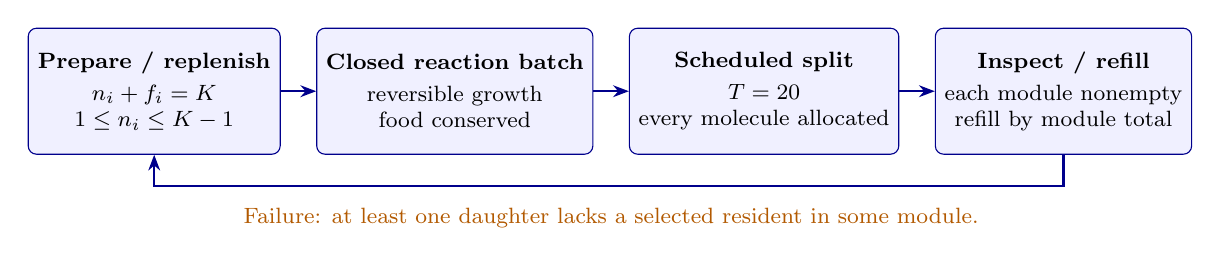
\begin{tikzpicture}[
  box/.style={draw=blue!55!black,fill=blue!6,rounded corners=3pt,minimum width=3.2cm,minimum height=1.6cm,align=center,font=\footnotesize},
  lab/.style={font=\small\bfseries,color=blue!55!black},
  arr/.style={-{Stealth[length=2mm]},thick,blue!55!black}]
\node[box] (a) {\textbf{Prepare / replenish}\\[2pt] $n_i+f_i=K$\\ $1\le n_i\le K-1$};
\node[box,right=0.45cm of a] (b) {\textbf{Closed reaction batch}\\[2pt] reversible growth\\ food conserved};
\node[box,right=0.45cm of b] (c) {\textbf{Scheduled split}\\[2pt] $T=20$\\ every molecule allocated};
\node[box,right=0.45cm of c] (d) {\textbf{Inspect / refill}\\[2pt] each module nonempty\\ refill by module total};
\draw[arr] (a) -- (b); \draw[arr] (b) -- (c); \draw[arr] (c) -- (d);
\draw[arr] (d.south) -- ++(0,-0.4) -| (a.south);
\node[font=\footnotesize,color=orange!70!black,anchor=north] at ($(b.south east)!0.5!(c.south west)+(0,-0.55)$) {Failure: at least one daughter lacks a selected resident in some module.};
\end{tikzpicture}}
\caption{One finite-food cycle. Each module conserves $K$ modelled molecules during the batch. Refill across both daughters adds exactly $K$ food molecules per module. The controller reads totals, never the encoded species identity.}
\label{fig:cycle}
\end{figure}

\section{Uniform finite-time copying}\label{sec:proof}

\subsection{The empty-daughter observable}
For $n\ge1$ put
\begin{equation}\label{eq:g}
 g(n)=2^{1-n},\qquad H(n_0,n_1)=g(n_0)+g(n_1),\qquad Q(n_0,n_1)=(1-g(n_0))(1-g(n_1)).
\end{equation}

\begin{lemma}[Exact partition law]\label{lem:partition}
Let a module hold $n\ge1$ residents at the split. The probability that daughter A receives none or all of them is exactly $g(n)$. Conditionally on the counts $(n_0,n_1)$ at time $T$, the probability that both daughters receive at least one resident of each module is exactly $Q(n_0,n_1)$, and $Q\ge1-H$.
\end{lemma}
\begin{proof}
The events that A receives zero or all $n$ molecules of the module are disjoint and each has probability $2^{-n}$, so their union has probability $2^{1-n}=g(n)$. Molecules of different modules are allocated independently, so the two module successes are conditionally independent given the counts and the joint success probability is the product $Q$. Finally $Q=1-H+g(n_0)g(n_1)\ge1-H$. No independence of the two count processes is used, only independence of the allocation of distinct molecules.
\end{proof}

The observable $H$ is thus an exact upper bound for the conditional failure probability, and a lower bound on $\EE_zQ(n(T))$ follows from an upper bound on $\EE_zH(n(T))$. The next lemma is the only piece of probability theory needed.

\begin{lemma}[Finite-state deadline bound]\label{lem:deadline}
Let $(Z_t)$ be a continuous-time Markov chain on a finite state space with generator $\cL$, and let $w\ge0$, $s>0$ and $\eta\ge0$ satisfy $\cL w\le-sw+\eta$ pointwise. Then for every start $z$ and $t\ge0$,
\begin{equation}\label{eq:expectation}
 \EE_z\,w(Z_t)\le e^{-st}w(z)+\frac{\eta}{s}\bigl(1-e^{-st}\bigr).
\end{equation}
\end{lemma}
\begin{proof}
On a finite state space $u(t)=\EE_zw(Z_t)$ is differentiable with $u'(t)=\EE_z\cL w(Z_t)\le-su(t)+\eta$ (Kolmogorov's backward equation, or Dynkin's formula \citep{ethierkurtz1986}). Multiplying $u'+su\le\eta$ by $e^{st}$ and integrating from $0$ to $t$ gives \eqref{eq:expectation}.
\end{proof}

In the formal development the finite-time law is defined as the matrix exponential $\bigl(e^{t\cL}h\bigr)(z)$ of the rate matrix, and Lemma~\ref{lem:deadline} is an instance of a residual certificate that combines a subsolution $v$ with $\cL v\ge-\varepsilon$, a decaying witness $w$ and a cover $v\le h+w$ (\lean{finite_deadline_residual_certificate}); here $v\equiv1$, $\varepsilon=0$, $h=Q$ and $w=H$.

\subsection{Local generator bounds}
Write $\cL$ for the generator of the count chain with rates \eqref{eq:birth}--\eqref{eq:death}. A birth in module $i$ multiplies $g(n_i)$ by $1/2$ and a death multiplies it by $2$, so
\begin{equation}\label{eq:local}
 \cL\,g(n_i)=n_i\,g(n_i)\,(1+\gamma n_j)\Bigl[b(n_i-1)-\frac a2(K-n_i)\Bigr],
\end{equation}
and the formula remains valid at $n_i=1$ and $n_i=K$ because the corresponding rates vanish there.

\begin{lemma}[Local generator bounds at the nominal rates]\label{lem:drift}
Let $(a,b,\gamma)=(1000,1,1/10)$ and $1\le n_i,n_j\le K$.
\begin{enumerate}[label=(\alph*)]
\item For $K=9$: $\ \cL g(n_i)\le-3900\,g(n_i)+\dfrac{2523}{160}$.
\item For $K=20$: $\ \cL g(n_i)\le-9000\,g(n_i)+\dfrac{2535}{131072}$.
\end{enumerate}
Both inequalities hold with equality at $n_i=n_j=K$.
\end{lemma}
\begin{proof}
(a) For $1\le n\le8$ the bracket in \eqref{eq:local} is $-[500(9-n)-(n-1)]$ and the function $n\mapsto n[500(9-n)-(n-1)]$ is a concave quadratic with endpoint values $4000$ at $n=1$ and $3944$ at $n=8$, hence at least $3944$ on the interior. Since $1+n_j/10\ge1$, the interior generator is at most $-3944\,g(n)\le-3900\,g(n)$. At $n=9$ the bracket is $8$, $g(9)=2^{-8}$ and $1+n_j/10\le19/10$, so
\[
 \cL g(9)+3900\,g(9)\le\frac{9\cdot8\cdot(19/10)+3900}{256}=\frac{2523}{160}.
\]
(b) For $1\le n\le19$ the quadratic $n[500(20-n)-(n-1)]$ has endpoint values $9500$ and $9158$, so the interior generator is at most $-9158\,g(n)\le-9000\,g(n)$. At $n=20$ the multiplier is at most $1+20/10=3$ and
$\cL g(20)+9000\,g(20)\le(20\cdot19\cdot3+9000)/2^{19}=2535/131072$.
\end{proof}

\subsection{The theorem}
\begin{theorem}[Finite-food copying]\label{thm:main}
Let $(a,b,\gamma)=(1000,1,1/10)$ and $T=20$. For $K=9$, every word $\sigma$ and every $z\in\cC_\sigma$, the complete cycle of Section~\ref{sec:cycle} satisfies
\begin{equation}\label{eq:q9}
 \PP_z\bigl\{Z_A^{\rm restart}\in\cC_\sigma\ \text{and}\ Z_B^{\rm restart}\in\cC_\sigma\bigr\}
 \ \ge\ q_9:=\frac{8046297159}{8112104000}>0.99188782 .
\end{equation}
For $K=20$ the same statement holds with
\begin{equation}\label{eq:q20}
 q_{20}:=\frac{7077818258231}{7077927321600}>0.99998459 .
\end{equation}
Admitted newborns carry at most $2(K-1)$ residents, and each compartment carries exactly $2K$ residents plus food at every time. Both bounds are uniform in the word and in the admitted state.
\end{theorem}
\begin{proof}
Fix $\sigma$ and $z\in\cC_\sigma$. By the invariance of the pure face and the generator identification, the resident counts at time $T$ are the counts $n(T)$ of the finite chain started at the selected counts of $z$. By Lemma~\ref{lem:partition} the conditional probability of a successful split is $Q(n(T))$; every successful split places both daughters on the pure face with counts in $\{1,\dots,K-1\}$, and the refill \eqref{eq:refill} is always possible and returns both to $\cC_\sigma$. Hence the joint-return probability equals $\EE_zQ(n(T))\ge1-\EE_zH(n(T))$.

Let $\cL g\le-sg+C$ be the local bound of Lemma~\ref{lem:drift}. Adding the two modules gives $\cL H\le-sH+2C$, and Lemma~\ref{lem:deadline} with $H(z)\le2$ yields
\[
 \EE_zH(n(T))\le2e^{-sT}+\frac{2C}{s}.
\]
The inequality $e^x\ge1+x$ gives $e^{-20s}\le(1+20s)^{-1}$. For $K=9$, $(s,C)=(3900,2523/160)$ and
\[
 \PP_z(\text{joint return})\ge1-\frac2{78001}-\frac{841}{104000}=q_9 .
\]
For $K=20$, $(s,C)=(9000,2535/131072)$ and the bound is $1-2/180001-169/39321600=q_{20}$. No terminal count is prescribed: a parent with food remaining at time $T$ is included with its actual partition probability. The molecule budgets follow from \eqref{eq:conservation} and the definition of $\cC_\sigma$.
\end{proof}

\begin{remark}
The argument uses the deadline only through $e^{-20s}\le1/78001$; the bound is dominated by the residual term $2C/s$, which comes entirely from the boundary state $n_i=K$ where births have stopped and only reverse reactions act. Any deadline $T\ge1/100$ would already give a bound above $0.99$ at $K=9$; the chosen $T=20$ makes the decaying term negligible and matches the companion protocol.
\end{remark}

\subsection{How tight is the bound?}\label{sec:tight}
The bound has two losses: replacing $Q$ by $1-H$, which costs $\EE\,g(n_0)g(n_1)\approx1.6\times10^{-5}$ at stationarity, and the Lyapunov residual $2C/s$, which exceeds the stationary value $2\EE_\pi g$ by a small amount because the boundary constant $C$ is evaluated at the worst neighbour count. Table~\ref{tab:tight} compares the proved bounds with floating-point evaluations of the one-cycle probability $\EE_zQ(n(T))$ from the matrix exponential of the $K^2\times K^2$ rate matrix, and with the exact stationary value $(1-\EE_\pi g)^2$ computed from the product law of Section~\ref{sec:stationary}. Both are diagnostics, not certificates. At $T=20$ every admitted start gives the same value to eleven digits, as expected for a chain whose rates are of order $10^3$ to $10^4$. The proved bound is within $2.5\times10^{-4}$ of the numerically evaluated probability at $K=9$ and within $1.2\times10^{-5}$ at $K=20$; the construction itself is within $7\times10^{-5}$ (respectively $8\times10^{-8}$) of the fair-partition ceiling $u_K=Q(K,K)$ that no dynamics on $\{1,\dots,K\}^2$ can exceed.

\begin{table}[t]
\centering\small
\caption{Proved bounds against numerical diagnostics. The middle column is $\EE_zQ(n(20))$ from the matrix exponential (minimum over admitted starts; the maximum agrees to $10^{-11}$); the stationary value is exact rational arithmetic rounded. Only the first column is a theorem.}\label{tab:tight}
\begin{tabular}{@{}lcccc@{}}
\toprule
$K$ & proved $q_K$ & numerical one-cycle return & stationary $(1-\EE_\pi g)^2$ & ceiling $u_K=Q(K,K)$\\
\midrule
$9$ & $0.99188782$ & $0.99213251$ & $0.99213251$ & $0.99220276$\\
$20$ & $0.99998459$ & $0.99999611$ & $0.99999611$ & $0.99999619$\\
\bottomrule
\end{tabular}
\end{table}

Figure~\ref{fig:traj} shows why the estimate is so close. Starting from the worst admitted state $(1,1)$, amplification to $K=9$ is complete within a few thousandths of a time unit: the birth rate at $n_i=1$ is $a(K-1)(1+\gamma n_j)\ge8800$. Thereafter the chain sits at $n_i=K$ with occasional single reverse steps, and $\EE_zH$ settles at $2\EE_\pi g=0.00788$, just below the proved floor $2C/s=0.00809$. Panel~(a) shows six Gillespie sample paths \citep{gillespie1977} together with the exact mean count; panel~(b) shows the exact $\EE_zH(n(t))$ for three starts against the envelope \eqref{eq:expectation}.

\begin{figure}[t]
\centering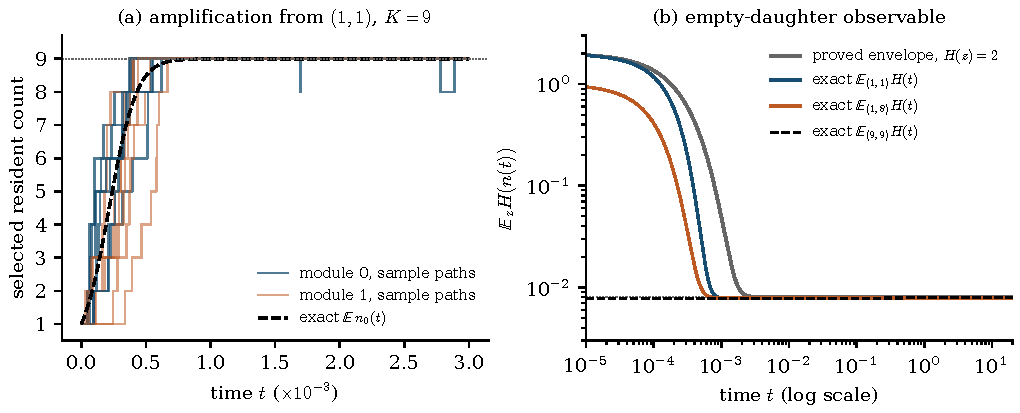
\includegraphics[width=\linewidth]{figures/trajectories.pdf}
\caption{Amplification and the empty-daughter observable at $K=9$, nominal rates. (a) Six Gillespie sample paths of the selected counts from the worst admitted start $(1,1)$ on the first $3\times10^{-3}$ time units, with the exact mean count $\EE\,n_0(t)$ from the matrix exponential (dashed). (b) Exact $\EE_zH(n(t))$ for the starts $(1,1)$, $(1,8)$ and $(9,9)$ on a logarithmic time axis, against the proved envelope $2e^{-3900t}+(2C/s)(1-e^{-3900t})$ and its floor $2C/s$ (dotted). Both panels are numerical illustrations of proved statements, not evidence used in a proof.}
\label{fig:traj}
\end{figure}

\section{An explicit operating region}\label{sec:box}
\begin{theorem}[Operating box]\label{thm:box}
Let $K=9$, $T=20$, and suppose
\begin{equation}\label{eq:box}
 500\le a\le1500,\qquad \tfrac12\le b\le2,\qquad \tfrac1{20}\le\gamma\le\tfrac29 .
\end{equation}
Then every admitted state of every word has joint-return probability at least
\begin{equation}\label{eq:qbox}
 q_{\rm box}:=1-\frac2{36001}-\frac{31}{3200}=\frac{114080769}{115203200}>0.99025694 .
\end{equation}
\end{theorem}
\begin{proof}
By \eqref{eq:local}, $\cL g(n)=n\,g(n)(1+\gamma m)\bigl[b(n-1)-\tfrac a2(9-n)\bigr]$ with $m$ the neighbour count. For $1\le n\le8$ the bracket is negative and is bounded above by $2(n-1)-250(9-n)$, obtained by replacing $a$ by $500$ and $b$ by $2$. The concave quadratic $n[250(9-n)-2(n-1)]$ has endpoint values $2000$ and $1888$, so with $1+\gamma m\ge1$ the interior generator is at most $-1888\,g(n)\le-1800\,g(n)$. At $n=9$ the bracket is $8b\le16$ and $1+\gamma m\le1+\tfrac29\cdot9=3$, so
\[
 \cL g(9)+1800\,g(9)\le\frac{2\cdot9\cdot8\cdot3+1800}{256}=\frac{279}{32}.
\]
The proof of Theorem~\ref{thm:main} with $(s,C)=(1800,279/32)$ gives \eqref{eq:qbox}.
\end{proof}

The generator inequality is affine in $a$ and in $b$ for fixed counts and $\gamma$, and affine in $\gamma$ for fixed counts, $a$ and $b$; the formal proof treats the three parameters symbolically over the whole box, and the exact replay of the vertex cases in \path{check_paper.py} is a diagnostic only. The uncertainty covered is within the compatible family \eqref{eq:reactions}: catalytic coefficients are $a\gamma$ and $b\gamma$, so the common ratio $a/b$ is preserved, and the box does not cover independently perturbed channel constants, additional reaction channels or contamination. Within the box the equilibrium ratio ranges over $[250,3000]$.

\section{The minimum peak budget}\label{sec:budget}
The construction at $K=9$ never holds more than $18$ residents. The following proposition shows that, within the architecture actually used, $18$ is also necessary, and that the constraint is combinatorial rather than dynamical: it comes from the fair split, not from the reaction kinetics.

\begin{proposition}[Restricted sharp budget]\label{prop:budget}
Consider any two-module pure-species architecture whose complete cycle allocates individual resident molecules independently and fairly to two complementary daughters, requires an immediate representative of each module in both daughters, and performs no resident repair. If the parent's resident total at the split is always at most $17$, the joint-return probability is strictly less than $0.99$, whatever the preceding dynamics and whatever the law of the parent state. Eighteen peak residents suffice in this class.
\end{proposition}
\begin{proof}
A parent with an empty module has zero success probability. Otherwise, by Lemma~\ref{lem:partition}, the conditional success probability given counts $(r,s)$ is $Q(r,s)=(1-2^{1-r})(1-2^{1-s})$, which is increasing in each argument. For a fixed total $r+s$ and $s\ge r+2$, direct subtraction gives
\[
 Q(r+1,s-1)-Q(r,s)=2^{-r}-2^{1-s}>0 ,
\]
so the balanced split maximizes $Q$ at a given total. Monotonicity lets any total below $17$ be raised to $17$, whose maximum is attained at $(8,9)$ or $(9,8)$:
\[
 Q(r,s)\le\frac{127}{128}\cdot\frac{255}{256}=\frac{32385}{32768}=0.988311767578125<0.99 .
\]
Taking the expectation over an arbitrary law of the parent counts preserves this pointwise ceiling. Sufficiency is Theorem~\ref{thm:main} at $K=9$, whose chain reaches $(9,9)$ by a positive-rate path, so the capacity $18$ is actually used.
\end{proof}

Figure~\ref{fig:budget} places the two proved points against the fair-partition failure floor $1-u_K=1-(1-2^{1-K})^2$ as a function of the peak capacity $2K$. The claim of Proposition~\ref{prop:budget} is restricted to the stated architecture; a mechanism with unequal or correlated allocation, with several representatives per label, or with repair after birth is outside its scope, as is any statement about a universal minimum molecule count for chemical memory.

\begin{figure}[t]
\centering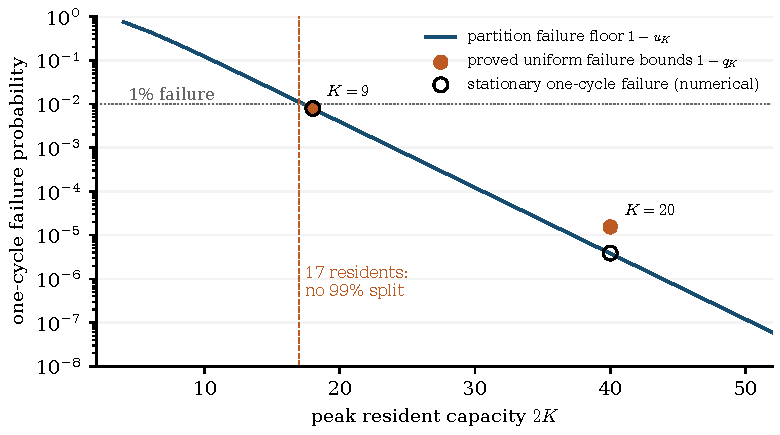
\includegraphics[width=.8\linewidth]{figures/budget.pdf}
\caption{Budget and fidelity. The curve is the exact fair-partition failure floor $1-u_K$ that no dynamics on $\{1,\dots,K\}^2$ can beat. Filled points are the proved uniform failure bounds $1-q_K$ for $K=9,20$; open circles are the stationary one-cycle failures from Table~\ref{tab:tight} (numerical). The dashed line marks the seventeen-resident ceiling of Proposition~\ref{prop:budget}. The gap between a filled point and the curve is the slack of the proof, not a simulation confidence interval.}
\label{fig:budget}
\end{figure}

\section{Composition geometry}\label{sec:geometry}
Normalize the four resident counts by their total, excluding food, to obtain the composition $p(z)\in\R^4$ of a state $z$. We show that the four admitted regions are separated in $L^1$ by exactly $2/K$ and that the readout is stable.

\begin{proposition}[Sharp composition margin]\label{prop:gap}
For every $K\ge2$,
\begin{equation}\label{eq:gap}
 \min_{\sigma\ne\tau}\ \inf_{z\in\cC_\sigma,\ z'\in\cC_\tau}\ \norm{p(z)-p(z')}=\frac2K ,
\end{equation}
and the minimum is attained. A nearest-region decoder returns the correct word from any measured composition within $L^1$ distance strictly less than $1/K$ of $p(z)$, $z\in\cC_\sigma$.
\end{proposition}
\begin{proof}
In an admitted state module $i$ holds at least one resident and the other module at most $K-1$, so the occupied coordinate of module $i$ satisfies $p_{S_i}(z)\ge1/K$. If $\sigma$ and $\tau$ differ in bit $i$, the coordinate occupied by $\sigma$ in module $i$ is zero in every state of $\cC_\tau$, and conversely, so these two coordinates contribute at least $1/K$ each to the $L^1$ distance, giving the lower bound $2/K$. Equality holds for two words differing only in module $i$, with $n_i=1$ and $n_j=K-1$ in both states: the two module-$i$ coordinates are $1/K$ and $0$ (in either order) and the module-$j$ coordinates coincide. For the decoder, if a measured composition $p'$ with $\norm{p'-p(z)}<1/K$ were at least as close to some $z'\in\cC_\tau$, $\tau\ne\sigma$, the triangle inequality would give $\norm{p(z)-p(z')}<2/K$, contradicting \eqref{eq:gap}.
\end{proof}

For $K=9$ the gap is $2/9$ and the tolerance $1/9$; for the count band $1,\dots,19$ of the earlier quenched construction the sharp gap is $1/10$. Word pairs differing in both modules may be farther apart; \eqref{eq:gap} is the global minimum. A fixed exact decoder simply tests which of the two species of each module has positive fraction (\lean{decode}); on the admitted regions the local alternative-species fractions are exactly zero or one. These are measurement guarantees and say nothing about a reaction system removing contaminating molecules.

\section{Repeated copying}\label{sec:repeat}
\subsection{The actual successful-restart kernel}
Let $\cA_K=\{1,\dots,K-1\}^2$ be the admitted selected counts and $P_T(x,n)$ the transition probability of the count chain over one batch. For $x,y\in\cA_K$ define
\begin{equation}\label{eq:kernel}
 W(x,y)=\sum_{n}P_T(x,n)\prod_{i=0}^{1}\Bigl[2^{-n_i}\binom{n_i}{y_i}\mathbf 1\{1\le y_i<n_i\}\Bigr].
\end{equation}
$W(x,y)$ is the probability that, starting from admitted counts $x$, the split is successful and daughter A restarts with counts $y$; the indicator tests both complementary daughters, food allocation has been summed out because its binomial law sums to one, and the refill fixes daughter A's full next-cycle state. Hence $\sum_yW(x,y)=\EE_xQ(n(T))$ is exactly the joint-return probability, and the missing mass is failure. By symmetry of the split the same kernel describes daughter B. This constructs the restart law from the protocol rather than positing a kernel with a desired reliability.

\subsection{A selected lineage}
\begin{proposition}[Finite-lineage retention]\label{prop:lineage}
Run the cycle repeatedly with fresh label-blind supplies and resets, inspect both daughters at every split, and follow daughter A. Let $q_K$ be a uniform one-cycle bound from Theorem~\ref{thm:main} or~\ref{thm:box} and $u_K=(1-2^{1-K})^2$. The probability $S_N(x)$ that the first $N$ cycles all succeed satisfies
\begin{equation}\label{eq:lineage}
 q_K^N\le S_N(x)\le u_K^N\qquad(x\in\cA_K),
\end{equation}
and the probability that the selected lineage never fails is zero.
\end{proposition}
\begin{proof}
By the Markov property at the restart states, $S_0=1$ and $S_{N+1}(x)=\sum_yW(x,y)S_N(y)$. Every row sum of $W$ lies between $q_K$ (the uniform theorem) and $u_K$ (since $n_i\le K$ and $Q$ is increasing, $Q\le Q(K,K)=u_K$). Induction gives \eqref{eq:lineage}. The events $\{$first $N$ cycles succeed$\}$ decrease in $N$, so their probabilities converge to the probability of eternal success, which is at most $\lim u_K^N=0$. No unconditional independence between generations is used.
\end{proof}

\begin{table}[t]
\centering\small
\caption{Selected-lineage and family bounds. Percentages are rounded evaluations of the exact bases $q_K$ and $u_K$.}\label{tab:lineage}
\begin{tabular}{@{}lcccc@{}}
\toprule
\multicolumn{5}{@{}l}{\emph{Selected lineage, Proposition~\ref{prop:lineage}}}\\
$K$ & cycles $N$ & lower bound $q_K^N$ & upper bound $u_K^N$ & \\
\midrule
$9$ & $100$ & $44.28\%$ & $45.71\%$ & \\
$20$ & $1000$ & $98.47\%$ & $99.62\%$ & \\
\midrule
\multicolumn{5}{@{}l}{\emph{Complete family, Corollary~\ref{cor:family}}}\\
$K$ & depth $N$ & cycles $2^N-1$ & lower bound & upper bound $u_K^{2^N-1}$\\
\midrule
$9$ & $3$ & $7$ & $94.32\%$ & $94.67\%$\\
$9$ & $5$ & $31$ & $74.85\%$ & $78.47\%$\\
$20$ & $10$ & $1023$ & $98.42\%$ & $99.61\%$\\
$20$ & $14$ & $16383$ & $74.76\%$ & $93.94\%$\\
\bottomrule
\end{tabular}
\end{table}

\subsection{A complete family}
In the multi-generation protocol each successful daughter becomes a separate compartment with its own supplies, and separate compartments evolve independently given their restart states. A \emph{family of depth $N$} consists of the $2^N-1$ cycles run by the founder and all its descendants down to depth $N-1$; it succeeds when every one of these cycles succeeds, so that all $2^N$ descendants at depth $N$ are admitted states of the founder's word.

\begin{corollary}[Family retention]\label{cor:family}
Under the assumptions of Proposition~\ref{prop:lineage}, the probability that a family of depth $N$ succeeds satisfies
\begin{equation}\label{eq:family}
 1-(2^N-1)(1-q_K)\ \le\ \PP(\text{family of depth $N$ succeeds})\ \le\ u_K^{\,2^N-1}.
\end{equation}
\end{corollary}
\begin{proof}
Order the $2^N-1$ internal nodes so that each node follows its ancestors. The family fails only if some node $v$ fails while all its strict ancestors succeeded; on that event $v$ is in an admitted state, and conditionally on the history up to the start of $v$'s cycle the failure probability of $v$ is at most $1-q_K$ by the uniform theorem and the Markov property at $v$'s restart state. Hence each such event has probability at most $1-q_K$, and the union bound gives the lower bound. For the upper bound, condition on all cycles but the last in the order: the last node's success has conditional probability at most $u_K$, so the family success probability is at most $u_K$ times the success probability of the remaining nodes, and induction gives $u_K^{2^N-1}$.
\end{proof}

Table~\ref{tab:lineage} and Figure~\ref{fig:lineage} give the numbers. Two objectives are visibly distinct: $K=9$ minimizes molecules while $K=20$ retains a label across thousands of cycles, and neither is close to indefinite retention. The family bound concerns all descendants; the lineage bound concerns one selected line while both daughters are inspected at each split.

\begin{figure}[t]
\centering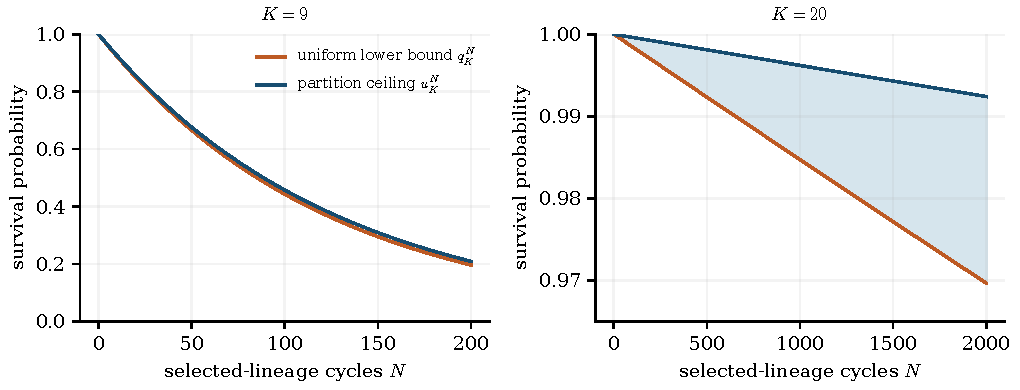
\includegraphics[width=\linewidth]{figures/lineage.pdf}
\caption{Selected-lineage bounds \eqref{eq:lineage}. The shaded band lies between the uniform lower guarantee $q_K^N$ and the partition ceiling $u_K^N$; axis ranges differ to show the two time scales. Neither curve assumes independence between generations.}
\label{fig:lineage}
\end{figure}

\section{Stationary law and label symmetry}\label{sec:stationary}
\begin{proposition}[Product-form stationary law]\label{prop:stationary}
Fix a word and put $R=a/b>0$. The one-module distribution
\begin{equation}\label{eq:stationary}
 \pi_K(n)=\frac{\binom Kn R^n}{(1+R)^K-1},\qquad 1\le n\le K ,
\end{equation}
is a probability law, and $\pi_K\otimes\pi_K$ is the unique stationary law of the count chain with rates \eqref{eq:birth}--\eqref{eq:death}, for every $\gamma\ge0$.
\end{proposition}
\begin{proof}
Normalization is the binomial theorem. Since $\pi_K(n+1)/\pi_K(n)=R(K-n)/(n+1)$, for every fixed neighbour count $m$
\[
 \pi_K(n)\pi_K(m)\cdot a\,n(K-n)(1+\gamma m)=\pi_K(n+1)\pi_K(m)\cdot b\,(n+1)n(1+\gamma m),
\]
so every edge of the chain satisfies detailed balance with respect to $\pi_K\otimes\pi_K$ \citep{kelly1979}. The chain on $\{1,\dots,K\}^2$ is irreducible for $a,b>0$, so the stationary law is unique.
\end{proof}

The catalytic factor $1+\gamma m$ multiplies both directions of every edge and cancels in the balance equation. Cross-catalysis therefore changes rates, trajectories and the transient law without changing the stationary law, and the factorization of $\pi$ does not imply independence of the two transient count processes. The calculation is consistent with the product-form theory for complex-balanced networks \citep{anderson2010}, which is not needed here. The stationary expectation $\EE_\pi g=\sum_n\pi_K(n)2^{1-n}$ is the exact rational number used in Table~\ref{tab:tight}; at $K=9$ it equals $0.0039415$, so the stationary one-cycle success is $(1-\EE_\pi g)^2=0.9921325$.

Permuting $X_i$ and $Y_i$ in either module preserves the reaction table, the partition rule and the refill. At matched count preparations the four words therefore have identical count-process and copying laws: the construction supplies inheritance without intrinsic fitness differences between its labels.

\section{Worked cycles, limitations and scope}\label{sec:limits}
\subsection{Two complete cycles at $K=9$}
\begin{example}
For word $01$ prepare $(4X_0,4Y_1;\,5F_0,5F_1)$: eight residents and ten food molecules. A possible parent state at the split has nine selected residents in each module and no food. One successful allocation is
\[
 \mathrm A=(4X_0,5Y_1),\qquad \mathrm B=(5X_0,4Y_1).
\]
Add food $(5,4)$ to A and $(4,5)$ to B. Each daughter restarts with module totals nine, and the total food added is eighteen.
\end{example}

\begin{example}
Complete conversion of food is not required. A parent $(7X_0,6Y_1;\,2F_0,3F_1)$ can split as
\begin{center}\small
\begin{tabular}{@{}lcccc@{}}
\toprule
 & $X_0$ & $Y_1$ & $F_0$ & $F_1$\\
\midrule
A & 3 & 2 & 1 & 2\\
B & 4 & 4 & 1 & 1\\
\bottomrule
\end{tabular}
\end{center}
with all other resident counts zero. Module totals are $(4,4)$ in A and $(5,5)$ in B; add food $(5,5)$ and $(4,4)$ respectively. The final food counts are $(6,7)$ and $(5,5)$, each module again holds nine modelled molecules, both daughters carry word $01$, and the total replenishment is still eighteen.
\end{example}

\subsection{A precise support limitation}
\begin{proposition}[Contamination is permanent]\label{prop:contamination}
Add one molecule of a previously absent resident species to a pure module and run the table \eqref{eq:reactions}. Then the count of that species remains positive for all time, and the probability that both daughters return to the original pure-label region in that cycle is zero.
\end{proposition}
\begin{proof}
A channel decreases the count of a species only through reverse autocatalysis, whose propensity contains the factor $n(n-1)$ and vanishes at $n=1$; catalytic appearances in other channels do not consume the species. Hence the count never returns to zero. At the split, at least one daughter receives at least one molecule of the alternative species, and the refill removes none, so that daughter is outside the original region.
\end{proof}

The mechanism thus lacks any active error correction: it tolerates dilution and partition losses, but not contamination through impure food, side reactions or mutation. The statement is restricted to the table \eqref{eq:reactions}; protocols with resident removal, conversion channels, mutation correction or a different admitted geometry are outside its scope, and designing a small-budget mechanism with common positive support and a positive mutation channel is the natural next question (Section~\ref{sec:discussion}).

\subsection{External operations and physical scope}
The eighteen-molecule accounting includes residents and food, not solvent, membranes, apparatus or the controller. The split is scheduled at a deterministic time, the allocation is perfectly fair and molecule-wise, and the refill requires an agent that measures the module totals $M_i^A,M_i^B$ and injects exactly the missing food without disturbing the residents. The volume reset is likewise ideal. The controller never reads which species is present, but it is external machinery, so the result is a benchmark for compartmentalized chemical memory under a stated protocol and not a model of an autonomous protocell. The trimolecular channels need an elementary realization before an experimental claim can be made (Remark~\ref{rem:bimolecular}); the rate constants and the time unit are hypothetical, and the equilibrium ratio $a/b=1000$ corresponds to a substantial free-energy drop per birth (Section~\ref{sec:thermo}) that the refilled food must carry. Thermodynamic consistency of the table does not quantify heat, work or the feasibility of the external operations.

\section{Discussion and open questions}\label{sec:discussion}
The paper answers a finite, quantitative question: two interacting reversible modules with nine modelled molecules each transmit four composition labels through a complete split-and-refill cycle with a uniform guarantee above $0.9918$, within $2.5\times10^{-4}$ of the numerically evaluated probability and within $7\times10^{-5}$ of the combinatorial ceiling, and no fair-split architecture of this kind can reach $0.99$ with fewer than eighteen peak residents. The proof is short because the observable is exact: $g(n)=2^{1-n}$ is the fair-partition failure probability, and the reaction table is arranged so that $g$ decays under the generator at rate thousands of times faster than the deadline.

Three limitations define the next questions. First, the labels occupy disjoint species supports and contamination is permanent; a mechanism whose four labels share a common positive support and survive a positive mutation or immigration channel would need a genuinely different restoring dynamics, and the balance between noise and restoration should be tested on a small model before any budget is claimed. Second, the split, the refill and the volume reset are external; replacing them by growth-driven division and a food-uptake channel changes the deadline, the conservation law and the admitted regions, and the immediate-return semantics used here would no longer apply unchanged. Third, the termolecular channels are effective rate laws; Remark~\ref{rem:bimolecular} shows which parts of the argument survive an explicit complex and which must be re-proved. None of these questions is answered by the present theorem, and none of the present bounds depends on their answers.

\appendix
\section{Formal verification and reproducibility}\label{app:verification}
The critical statements are checked in Lean~4 (toolchain \lean{leanprover/lean4:v4.30.0}) against a frozen Mathlib manifest \citep{demoura2021,mathlib2020}. Verification treats compiler warnings as errors and rejects any declaration depending on \lean{sorry}. The root file \lean{proofs/SmallResidentCompositionCopying/Publication.lean} exports three declarations. All three live in the namespace \texttt{SmallResident\allowbreak Composition\allowbreak Copying.\allowbreak FiniteFood}, and their content is as follows.
\begin{itemize}
\item \lean{publication}: for every word and admitted state at $K=9$, the actual return probability is at least $8046297159/8112104000$; on the operating box it is at least $114080769/115203200$; distinct words have composition distance at least $2/9$; newborns have at most $16$ and all states at most $18$ residents;
\item \lean{return20}: the $K=20$ bound $7077818258231/7077927321600$;
\item \lean{literal_next}: every positive-rate channel of the twenty-four-channel chemistry has the literal molecular stoichiometry of \eqref{eq:reactions}.
\end{itemize}
The machine-readable receipt records exit code zero, $18$ transitive dependency modules with matching source and artifact hashes, a verification time of $60.031$ seconds, and an axiom inventory consisting only of \lean{Classical.choice}, \lean{Quot.sound} and \lean{propext}; no native evaluation is used. The root source has SHA-256 \texttt{d111998e\ldots}; the frozen manifest has SHA-256 \texttt{a8df0b60\ldots}. The earlier quenched construction and its receipts are not in the dependency graph of the root.

\begin{center}\small
\begin{longtable}{@{}>{\raggedright\arraybackslash}p{.30\linewidth}>{\raggedright\arraybackslash}p{.64\linewidth}@{}}
\toprule Paper statement & Lean declarations and status\\\midrule\endhead
Reaction table, count chain, generator identification, Section~\ref{sec:model} & \lean{FiniteFoodSource}: \lean{conserved}, \lean{channel_sum}, \lean{generator_identification}, \lean{word_law}. The chemistry is a jump model on $\mathrm{Fin}\,4\times\mathrm{Bool}\times\mathrm{Option}\,\mathrm{Bool}$ (24 channels) with literal propensities; its finite-time law equals that of the aggregated chain for every word.\\[3pt]
Literal stoichiometry, invariance of the pure face & \lean{FiniteFoodInvariants}: \lean{literal_next}, \lean{food_transition}, \lean{absent_stays_absent}, \lean{resident_never_zero}.\\[3pt]
Lemma~\ref{lem:partition} & \lean{FiniteFoodPartition}: \lean{single_return} (the fair binomial sum minus its two endpoints equals $1-2^{-n}$), \lean{actual_payoff}, \lean{actual_return}.\\[3pt]
Lemma~\ref{lem:deadline} & \lean{CompositionalMemory.finite_deadline_residual_certificate} on the matrix-exponential law \lean{finiteTimeExpectation}; specialized in \lean{FiniteFoodDrift.deadline} with the bound $1-2/(20s+1)-2C/s$ and \lean{exp_bound} for $e^{-20s}\le1/(20s+1)$.\\[3pt]
Lemma~\ref{lem:drift} and Theorem~\ref{thm:main} & \lean{FiniteFoodDrift}: \lean{generator_H}, \lean{reward_cover}, \lean{local9}, \lean{local20}, \lean{nominal9}, \lean{nominal20}; \lean{FiniteFoodPartition}: \lean{return9}, \lean{return20}, \lean{refill}, \lean{admitted_daughters}, \lean{food_refill}.\\[3pt]
Theorem~\ref{thm:box} & \lean{FiniteFoodRobustness}: \lean{OperatingBox}, \lean{robust_local}, \lean{robust9}, \lean{positive_coefficients}, \lean{common_ratio}; \lean{FiniteFoodPartition.return_box}. Parameters are symbolic over the box.\\[3pt]
Proposition~\ref{prop:gap}, budgets, decoder & \lean{FiniteFoodGeometry}: \lean{budgets}, \lean{occupied}, \lean{separated} (lower bound $2/K$), \lean{decode}. The attainment of $2/K$ is the elementary example in the text.\\[3pt]
Proposition~\ref{prop:budget}; kernel \eqref{eq:kernel}; Proposition~\ref{prop:lineage}; Corollary~\ref{cor:family}; Proposition~\ref{prop:stationary}; label symmetry; Proposition~\ref{prop:contamination}; Remark~\ref{rem:bimolecular} & \emph{Conventional proofs} in the text, not separately Lean-verified. Their constants are replayed in exact arithmetic by \path{check_paper.py}.\\[3pt]
Table~\ref{tab:tight}, Figure~\ref{fig:traj}, open circles in Figure~\ref{fig:budget} & Floating-point matrix exponentials and Gillespie sample paths in \path{check_paper.py}; diagnostics, not certificates.\\
\bottomrule
\end{longtable}
\end{center}

\paragraph{Reproduction.}
From the repository root, through the proof bridge that fixes the frozen Mathlib project and does not update dependencies:
{\footnotesize\begin{verbatim}
python scripts/verify_proof.py \
    proofs/SmallResidentCompositionCopying/Publication.lean --timeout 600 \
    --declaration SmallResidentCompositionCopying.FiniteFood.publication \
    --declaration SmallResidentCompositionCopying.FiniteFood.return20 \
    --declaration SmallResidentCompositionCopying.FiniteFood.literal_next
\end{verbatim}}
The manuscript sources include \path{check_paper.py}, which asserts every printed constant (the generator inequalities on all $81$, $400$ and $648$ state or vertex cases, the rational bounds $q_9$, $q_{20}$, $q_{\rm box}$, the seventeen-resident ceiling, the sharp gaps $2/9$ and $1/10$, detailed balance on every edge, the lineage and family percentages and the two worked cycles) in exact rational arithmetic, evaluates the diagnostics of Table~\ref{tab:tight}, and draws Figures~\ref{fig:traj}--\ref{fig:lineage}. Its last run reported every check passed.

\bibliographystyle{plainnat}
\bibliography{refs}
\end{document}
